In the previous chapters collocation-based and Kriging surrogates were applied to several play problems in hopes of demonstrating the surrogates' efficacy. Ultimately, the same surrogate methods will be applied to a difficult problem in nuclear fuel performance modeling. Specifically, modeling the depletion behavior of high burnup fuel is of interest. The field of fuel performance modeling is an ideal application for surrogates because most modern fuel performance codes such as Bison \cite{Williamson} are computationally expensive and there is a relative abundance of experimental data to complement the computer codes. Recall that the true promise of surrogates arises when thousands of simulations of an expensive computer code are required, as is the case for optimization and calibration studies. The idea is to fold together computer simulations and experimental data to improve the computer code's predictive accuracy.    

Calibration studies involving the fuel performance code Bison have already been conducted by Swiler et. al. in \cite{Swiler2}. In \cite{Swiler2}, an optimal fuel relocation activation parameter is identified by an aggregated calibration to experimental observations of several Halden fuel rods. Surrogates were not required for the calibration study due to the relative simplicity of the fuel rod model used. The Dakota \cite{dakota} framework was used to complete the calibration study.       

For the proposed thesis research the application of interest arises from the extensive validation base for fuel performance modeling found in the Fumex-II database \cite{fumex2}. 
Specifically, the application involves calibrating fission gas parameters involved in modeling the Ris\o~ AN3 experiment since these parameters are notoriously uncertain. The Ris\o~ AN3 experiment consists of a base irradiation of four reactor cycles up to some 41 GWd/t, as shown in Fig. \ref{fig:riso_base_irradiation}, followed by a power ramp. The base irradiation takes place in the Biblis A pressurized water reactor \cite{fumex2}. 
\begin{figure}
\caption{\label{fig:riso_base_irradiation}
Base irradiation history for the Ris\o~ AN3 experiment.}
 \begin{center}
  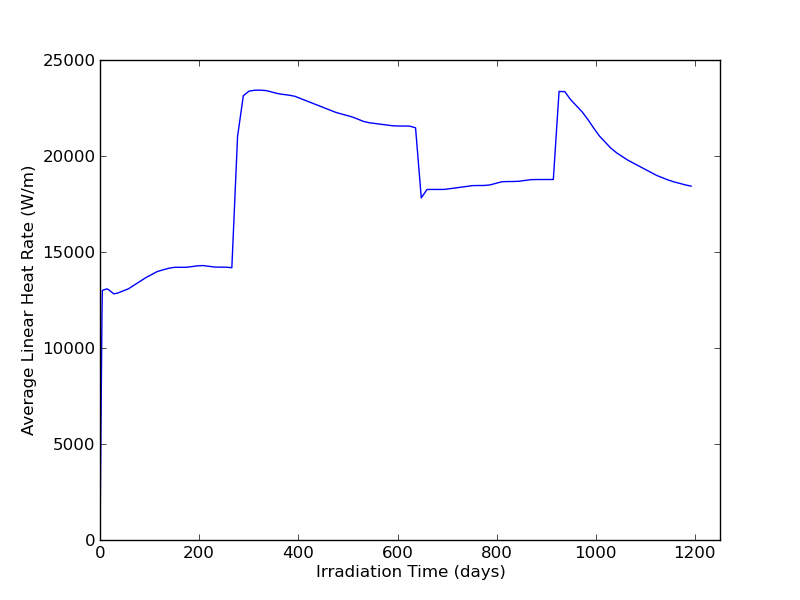
\includegraphics[scale=.75]{./Chapter4/base_irrad.png}
 \end{center}
\end{figure}     
After the base irradiation period, a fuel rod is extracted and refabricated to a shorter length before undergoing the power ramp in Fig. \ref{fig:riso_power_ramp}. The refabricated fuel rod was outfitted with various instrumentation such that fuel centerline temperature, fission gas release and rod internal pressure measurements could be obtained.  
\begin{figure}
\caption{\label{fig:riso_power_ramp}
Power ramp experiment for the the Ris\o~ AN3 experiment.}
 \begin{center}
  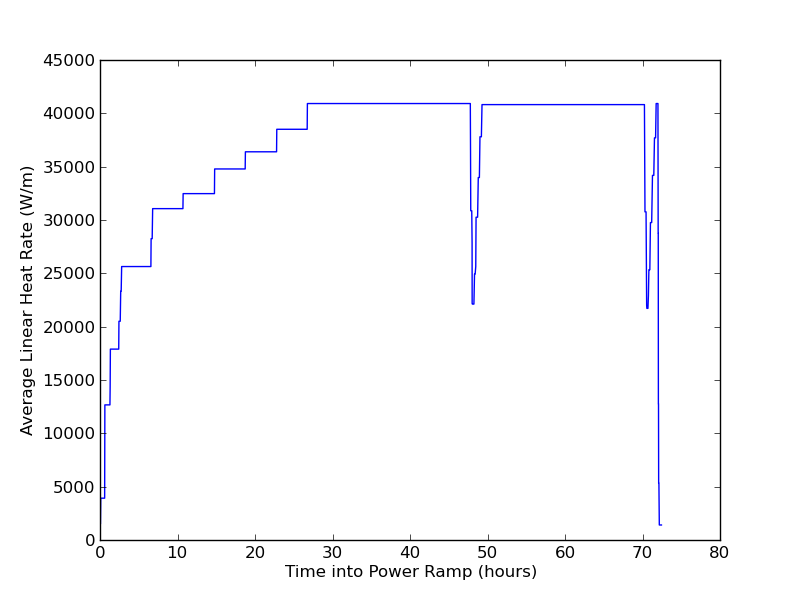
\includegraphics[scale=.75]{./Chapter4/power_ramp.png}
 \end{center}
\end{figure} 
The Ris\o~ AN3 test rod specifications are summarized in Table \ref{table:riso_specs}. The reader is encouraged to consult \cite{Perez2} for more in-depth specifications and modeling details.  

\begin{table} 
\caption{Ris\o~ AN3 test configurations and operating conditions.}
\label{table:riso_specs} 
\centering
\begin{tabular}{||c|c|c||} 
\hline \hline
\textbf{Description} & \textbf{Units} & \textbf{Value} \\ \hline
Overall fuel rod length & m  & 0.39058 \\ \hline
Fuel stack length        & m &  0.286 \\ \hline
Nominal plenum height  & mm & 61.0  \\ \hline
Pre-ramp rod fill gas composition & & He \\ \hline
Pre-ramp rod fill gas pressure & MPa & 2.31 \\ \hline
Refabfricated rod fill gas composition & & He \\ \hline
Refabfricated rod fill gas pressure & MPa & 1.57 \\ \hline
Fuel material    & & UO$_2$ \\ \hline
Fuel enrichment & \% & 2.95 \\ \hline
Fuel density      & \% & 93.74 \\ \hline
Fuel inner diameter   & mm & 2.5 \\ \hline
Fuel outer diameter   & mm & 9.053 \\ \hline
Pellet dish diameter   & cm & 0.665 \\ \hline
Pellet dish depth       & cm & 0.013 \\ \hline
Pellet chamfer width  & cm & 0.046 \\ \hline
Pellet chamfer depth  & cm & 0.016 \\ \hline
Cladding material          &  & Zr-4 \\ \hline
Cladding outer diameter  & mm & 10.81 \\ \hline
Cladding inner diameter   & mm & 9.258 \\ \hline
Cladding wall thickness   & mm &  0.776 \\ \hline
Base irradiation coolant inlet temperature & C & 287.7 \\ \hline
Base irradiation coolant pressure & MPa & 15.52  \\ \hline 
Power ramp coolant pressure & MPa & 15.3  \\ 
\hline \hline
\end{tabular}
\end{table}

The Ris\o~ AN3 experiment was modeled using solely Bison in \cite{Perez} and is included as a validation case for the Bison code. The relevant Bison input file and pertinent operating conditions, as utilized in this thesis, are included in Appendices \ref{app:bison_riso_input}, \ref{app:bison_operating_conds}. Note, the Bison Ris\o~ AN3 model is based upon the conditions and specifications in Table \ref{table:riso_specs} and \cite{Perez2}. To model fission gas release the \ac{SIFGRS} model is utilized in Bison. Bison's prediction of fission gas release during the power ramp is displayed alongside the corresponding experimental results in Fig. \ref{fig:riso_fgr}.  
\begin{figure}
\caption{\label{fig:riso_fgr}
Comparison of Bison fission gas release prediction to experimental results during the Ris\o~ AN3 power ramp.}
 \begin{center}
  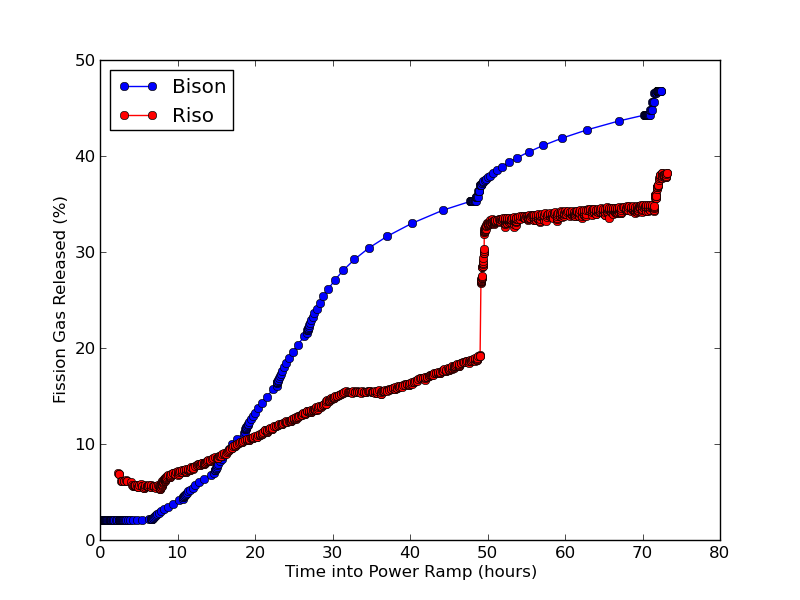
\includegraphics[scale=.75]{./Chapter4/fgr_comparison.png}
 \end{center}
\end{figure} 
As seen in Fig. \ref{fig:riso_fgr}, Bison over predicts fission gas release by a factor of two some forty hours into the power ramp. Similarly, Bison's prediction of fuel centerline temperature is plotted against experimental data in Fig. \ref{fig:riso_tc_temp}. Since fission gas release and fuel temperature are strongly coupled \cite{Perez}, it is anticipated that better fission gas release predictions will result in a more accurate fuel centerline temperature comparison. 

Calibrated parameters in \ac{SIFGRS} are expected to decrease the error between Bison's predicted output and the experimental data. Input parameters to \ac{SIFGRS} such as the fuel grain radius, hydrostatic stress, fuel porosity, bubble surface tension, and the gas diffusion coefficient are quite generic and uncertain. Consequently, adjusting such parameters to better match experimental data is justified. However, Bison's fission gas release predictions are computationally expensive. Considering the calibration of parameters in \ac{SIFGRS} will requires thousands of Bison instances, a surrogate model for fission gas release behavior becomes necessary. 
\begin{figure}
\caption{\label{fig:riso_tc_temp}
Comparison of Bison fuel centerline temperature prediction to experimental results during the Ris\o~ AN3 power ramp.}
 \begin{center}
  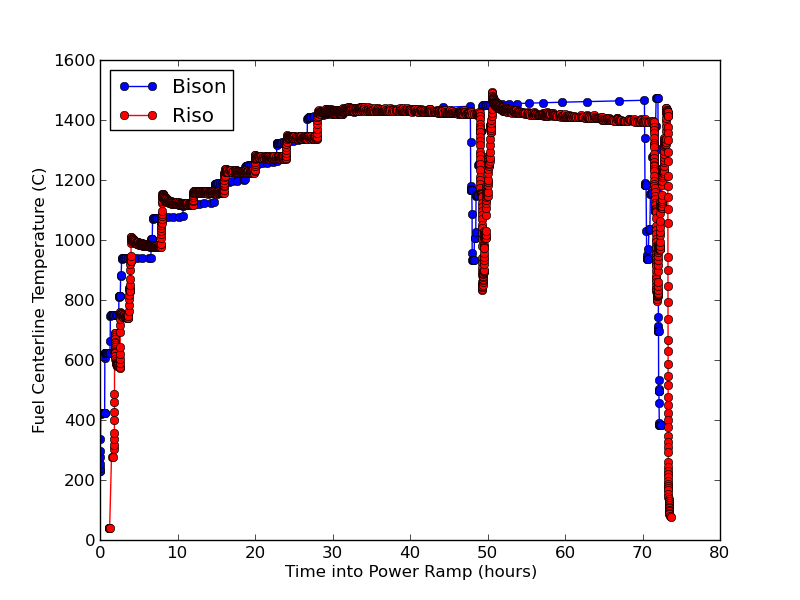
\includegraphics[scale=.75]{./Chapter4/tc_temp_comparison.png}
 \end{center}
\end{figure} 
As in \cite{Swiler}, the Dakota framework will be utilized to construct surrogate models for fission gas release behavior and to perform calibration routines. 

The primary culprits in the \ac{SIFGRS} model have been identified in \cite{Swiler3} and \cite{Pastore} to be the initial fuel grain radius, fuel porosity, surface tension, temperature, fuel grain radius, diffusion coefficient, resolution parameter and grain boundary coefficient. The importance and role of of these variables will be described in section \ref{sec:fgrTheory}. For now, suffice it to say that the true values of these variables are unknown and only uniform probability distributions can be attached to each variable. As a starting point for analysis, the \ac{LHS} module in Dakota was utilized to sample the variable space and simulate the resulting fission gas release time series resulting from the Ris\o~ AN3 power ramp. The 100 resulting time series are shown in Fig. \ref{fig:fgrSimulations}.
\begin{figure}
\caption{\label{fig:fgrSimulations}
Fission gas release time series for 100 \ac{LHS} Bison simulated Ris\o~ AN3 power ramp experiments.}
 \begin{center}
  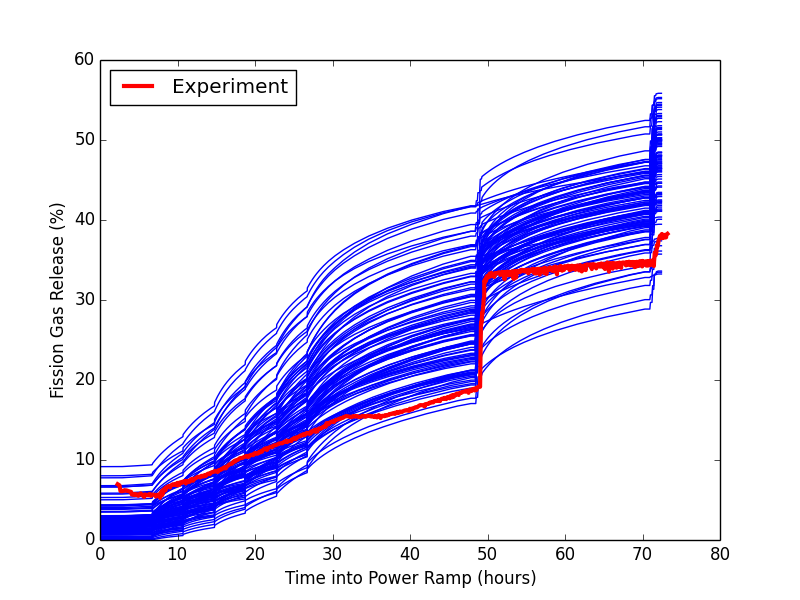
\includegraphics[scale=.75]{./Chapter4/fgr_simulations.png}
 \end{center}
\end{figure}
From Fig. \ref{fig:fgrSimulations}, it is clear that Bison tends to over predict fission gas release. However, it is also apparent that the range of variables is sufficient to contend with the experimental data.

The problem of finding "true" fission gas release parameters that will yield a release profile similar to that provided by experimental data is complicated by the quality of the experimental data. As seen in Fig. \ref{fig:riso_fgr}, the fission gas release is not monotonically increasing at all time steps in the power ramp. Of course, such a result is not physical. One possible explanation for the fission gas release decrease attributes the pressure transducers used to measure plenum pressure. Under some conditions released fission gases get trapped in fuel gaps and cracks, thereby not contributing to plenum pressure. The same phenomenon is believed to cause the large release of fission gas occurring at approximately hour fifty into the power ramp \cite{Pastore1}. Observe the large drop in power occurring at the same time as the spike in rod internal pressure measured by the transducer. As the power drops the cracks where fission gases are stored open. Consequently, although such fission gases were actually released earlier in the power ramp, the pressure transducer registers the gases in one burst. A burst of fission gases is expected to occur in the event of pellet-clad mechanical interaction. However, no such interaction took place during the Ris\o~ AN3 power ramp. The fission gas burst is controversial and currently not well understood \cite{Pastore1}. An alternative explanation suggests the burst is caused by gases accumulated at grain boundaries. Given the active research and discussion in this area, it is safe to say the fission gas release model implemented in Bison is not capable of exactly reproducing experimental observations. Indeed, no fission gas release burst mechanism exists in the Bison code. Such shortcomings will have to be considered when performing calibration on fission gas parameters.    



